% !TEX TS-program = pdflatex
% !TEX encoding = UTF-8 Unicode

\documentclass[12pt]{article}
%\documentclass[10pt,twocolumn]{article}

\usepackage[utf8]{inputenc} % set input encoding (not needed with XeLaTeX)

%%% PACKAGES
\usepackage{amsmath}
\usepackage{amsfonts}
\usepackage{graphicx}
\usepackage{booktabs}	 % for much better looking tables
\usepackage{array}	 % for better arrays (eg matrices) in maths
\usepackage{breqn} 	% breaks lines
\usepackage{authblk}	% helps with authors on title page
\usepackage{multirow}
% \usepackage{fancyhdr}
\usepackage{csquotes}
\usepackage[font={small,it}]{caption}

%\pagestyle{fancy}
%
%\lhead{}
%\chead{}
%\rhead{}


%----------------------------------------------------------------------------
\begin{document}
\pagenumbering{gobble}
%----------------------------------------------------------------------------
\renewcommand\Authfont{\small}
\renewcommand\Affilfont{\itshape\footnotesize}
%----------------------------------------------------------------------------
\title{
	{Educational Scheduling as a Mixed Integer Programming Model}\\
	\vspace{2cm}
	{\large Final Paper for ETM 540 (Fall 2016)}\\
	{\large Taught by Professor Tim Anderson, Ph.D.}\\
	\vspace{2cm}
}

% \title{Educational Scheduling as a Mixed Integer Programming Model}


%----------------------------------------------------------------------------
\author[1,2]{Will Kearney}
\author[1,2]{Sonimar Poppe}
\author[2]{Niguel Morfin}
\author[2]{Asrar Ahmed Syed}
\affil[1]{Portland Public Schools}
\affil[2]{Engineering and Technology Management, Portland State University}
%----------------------------------------------------------------------------
%\date{} % Activate to display a given date or no date (if empty),
         % otherwise the current date is printed 
%----------------------------------------------------------------------------

\maketitle
\newpage

\begin{abstract}
In this paper, we present an application of using Mixed Integer Programming (MIP) to schedule classes for a middle school in Portland, Oregon. This case study helps demonstrate that mathematical programming is an effective method for solving the educational timetabling problem. Furthermore, we demonstrate that mathematical programming is a particularly useful tool when school administrators need to quickly model school schedules in response to shifting enrollment, changing educational legal requirements, and other problems that can potentially be mediated through more efficient scheduling.
\end{abstract}

\newpage

\tableofcontents
\newpage

\pagenumbering{arabic}

\section{Introduction}

\subsection{The Educational Scheduling Problem}

The educational scheduling problem is a subset of the more general timetabling problem. In Kristiansen (as cited in \cite{wren1995scheduling}) timetabling is defined as:

\begin{displayquote}
Timetabling is the allocation, subject to constraints, of given resources to objects being placed in space time, in such a way as to satisfy as nearly as possible a set of desirable objectives. \cite{kristiansen2013comprehensive}
\end{displayquote}

Computer solutions to timetabling has existed in the literature since 1950 \cite{wren1995scheduling}, though it is not until recently that increased computing power and algorithmic improvements (namely improved in linear programming search heuristics, such as the so-called feasibility pump \cite{Fischetti2005}) has allowed mathematical formulations to successfully produce timetabling solutions in reasonable timeframes.

As a subset of the timetabling problem, educational scheduling has correspondingly benefited from these computional speed-ups. For example, Martin \cite{martin2004ohio} describes using integer programming to schedule classes at Ohio University’s College of Business; more recently, Schimmelpfeng \cite{schimmelpfeng2007application} uses an integer programming approach to create the complete timetable for all courses for a term at Hannover University, Germany.

Computational approaches become increasingly appealing when we consider how educational timetabling is often currently performed. For example, PowerSchool offers multiple-day on-site workshops designed to teach administrative staff how to design master schedules based on a complex iterative---and ultimately heuristic---approach \cite{powerSchool}. While certainly capable of producing feasible solutions, these approaches do not gaurantee optimality (however that is defined) and are very time intensive and expensive. Furthermore, these approaches do not lend themselves easily to exploring different scheduling objectives or modeling various scenarios due to the time involved in producing a schedule.

\subsection{Why is Educational Scheduling Important?}

Efficient educational scheduling allows schools to cope with a wide variety of changes. For example, almost all public schools eventually deal with issues of under- and over-enrollment as population shifts occur within school district boundaries. Appropriate school scheduling is one of many ways a school district can cope with changes in enrollment by optimizing resources such as teachers, staff members, and classrooms.
The constantly changing legislative landscape also requires schools to respond to local-, state-, and federally-mandated educational requirements. Often, these educational requirement require direct changes to students schedules.

\section{Problem Statement}

In this paper, we perform a case study on a middle school in Portland, Oregon currently experiencing over-enrollment. Additionally, the Governor of Oregon signed House Bill 3141 into law, requiring that students in grades six through eight receive 225 minutes of physical education (PE) per week; this translates to 45 minutes per day \cite{HouseBill3141}. Schools must be in compliance by the 2017-18 school year, and no additional funding is provided by the state.

Taken together, these challenges present a unique opportunity to demonstrate the ability of Mixed Integer Programming to aid in educational scheduling. Specifically, we create two models: the first model seeks to lower class sizes while ignoring the new PE requirements, while the second model incorporates all elements of the first while further incorporating the daily PE requirement into students' schedules.

\subsection{Assumptions}

We make a number of assumptions in order to simplify the problem description, but we believe these assumptions are reasonable and do not detract from the validity of our conclusions. First, we assume that each student must take the same ``core'' classes that she is currently enrolled in. Core classes are the set of courses in common subject areas---such as English language arts, math, science, and social studies---required of all middle school students. They are distinct from electives such as music and art.

Second, we analogously assume that teachers can only teach the courses they are currently taking. These are the only courses to which they can be assigned in the mathematical model (though they might not be assigned to \textit{all} of the same courses, and the number of sections of each might differ substantially).

Third, we assume each course has an upper bound equal to the number of students currently enrolled in that course \textit{or} 30, whichever is lower. Some support courses, such as Special Education, have very low upper bounds.

Fourth, we assume students desire to take the same electives they are currently enrolled in. Of course, it is possible that some students are forced to take particular electives because of the nature of their current schedule. If a MIP model were actually used to schedule a school, students could rank their desired electives in order of preference, which could then be incorporated into the objective function. Essentially, we are using students' current elective choices as a proxy for their hypothetical preference ranking.


\section{Our Approach}

Our implementation centered around a Python script that was used to pull in data directly from the Portland Public Schools relational database. All names were anonymized in the process.

We used Python as an algebriac modeling language and solved the resulting set of linear equations using Gurobi Optimizer, a state-of-the-art mathematical programming solver \cite{gurobi}.


\section{Model Formulation}


\subsection{Decision Variables}

\begin{table}[]
\centering
\caption{The data notation used in our formulation}
\label{tab:data-notation}
\begin{tabular}{ll}
\hline
$maxClassSize_{c}$ & Maximum number of students \\
 & permitted in class $c$ \\
$maxNumPeriods_{t}$ & Maximum periods teacher $t$ can teach\\
$enrolled_{s,c}$ & If student $s$ is currently taking course $c$\\
$core_{c}$ & Indicator is course $c$ is a core course \\
$PE_{c}$ & Indicator is course $c$ qualifies as physical education \\
$FTE_{c}$ & The amount of FTE for teacher $t$ \\
\hline
\end{tabular}
\end{table}

\begin{table}[]
\centering
\caption{The index notation used in our formulation}
\label{tab:index-notation}
\begin{tabular}{ll}
\hline
$s$ & $\in$ Set of students \\
$t$ & $\in$ Set of teachers \\
$c$ & $\in$ Set of courses \\
$p$ & $\in$ Set of periods \\
\hline
\end{tabular}
\end{table}

We used a set of decision variables to indicate if students and teachers were assigned to courses in various periods as follows:

% student decision variables
\begin{equation}
	X_{s,c,p} = 
	\begin{cases}
		1, & \text{if student}\ s \text{ is assigned to course}\ c \text{ in period}\ p	\\
		0, & \text{otherwise}
	\end{cases}
\end{equation}

and

% staff decision variables
\begin{equation}
	Y_{t,c,p} = 
	\begin{cases}
		1, & \text{if teacher}\ t \text{ is assigned to course}\ c \text{ in period}\ p	\\
		0, & \text{otherwise}
	\end{cases}
\end{equation}

Additionally, we used a set of binary variables $Z_{t}$ to indicate if teacher $t$ is teaching at all.

% Z indicator var
\begin{equation}
	Z_{t} = 
	\begin{cases}
		1, & \text{if teacher}\ t \text{ is teaching}	\\
		0, & \text{otherwise}
	\end{cases}
\end{equation}


\subsection{General Constraints}

The first constraint set is general in that it guarantees some basic conditions regardless of any other criteria that may be additionally required; it is the ``base model'', so to speak.

\begin{equation} \label{eq:every-student-fully-scheduled}
	\displaystyle \sum_{c} X_{s,c,p} = 1 \quad \forall s,p
\end{equation}

Constrainst~\ref{eq:every-student-fully-scheduled} ensures that every student is full scheduled (i.e. taking exactly one course every period of the day); for each student and period, the sum across all the courses must be equal to one.

\begin{equation} \label{eq:double-book-teachers}
	\displaystyle \sum_{c} Y_{t,c,p} \leq 1 \quad \forall t,p
\end{equation}

Similarly, constrainst~\ref{eq:double-book-teachers} ensures that no teachers are double-booked; in other words, each teacher can be assigned to at maximum one course during each period. Note that this doesn't exclude multiple teachers from being assigned the same course during the same period; this is what permits multiple class sections to exist during the same period.

\begin{equation} \label{eq:only-one-class}
	\displaystyle \sum_{p} X_{s,c,p} \leq 1 \quad \forall s,c
\end{equation}

Constraint~\ref{eq:only-one-class} guarantees that a student can't take a given class more than once per day.

\begin{equation} \label{eq:lunch-constraint}
\begin{split}
	X_{s,lunch,3} + X_{s,lunch,4} = 1 \quad \forall s \\
	Y_{t,lunch,3} + Y_{t,lunch,4} = Z_{t} \quad \forall t
\end{split}
\end{equation}

Every student and teacher should be scheduled to lunch in one of two lunch periods. In a 7 period day, lunch periods are 3 and 4; in an 8 period day, lunch periods are 4 and 5. Constraint~\ref{eq:lunch-constraint} illustrates a 7 period day.


\subsection{Capacity}

Most obviously, capacity can be thought of in terms of the number of students assigned to a particular class and period. The maximum number of students allows in a class is denoted by $maxClassSize_{c}$, which has an upper bound of 30, though it is often lower. Class size capacity is enforced as follows:

\begin{equation} \label{eq:class-size-capacity}
	\displaystyle \sum_{s} X_{s,c,p} \leq maxClassSize_{c} \cdot \displaystyle \sum_{t} Y_{t,c,p} \quad \forall c,p
\end{equation}

Constraint~\ref{eq:class-size-capacity} restricts the maximum number of students assigned to a class and period to the maximum number of seats available. It is important to recognize that multiple sections of a course can be taught during the same period, which is why equation~\ref{eq:class-size-capacity} includes the decision variable $Y_{t,c,p}$. Because the maximum class size is multiplied by the number of teachers assigned to that course and period, an arbitrary number of teachers can be assigned to help reduce class size by increasing the number of sections (subject to teacher availability constraints, of course).

Capacity can also be thought of in terms of the numbers of courses each teacher can be assigned. Largely, this is dictated by financial constraints. Teachers workloads are permitted on the basis of full-time equivelent (FTE) units; an FTE of 1 is equivalent to a full-time teacher, or 40 hours per week. Additionally, full-time teachers are required to have at least one planning period per day.

\begin{table}[]
\centering
\caption{The maximum number of periods a teacher is allowed to teach, based on their FTE workload and the number of periods in the day. For example, in a 7 period schedule, a teacher with FTE 0.75 can teach a maximum of 5 periods. This is an approximate simplification of actual PPS contractual limits that delineate the number of courses that can be taught per FTE.}
\label{tab:max-num-periods}
\begin{tabular}{lcccc}
             & \multicolumn{4}{c}{FTE} \\ \cline{2-5} 
             & 0.25 & 0.5 & 0.75 & 1.0 \\ \cline{2-5} 
7 period day & 1    & 3   & 5    & 6   \\
8 period day & 2    & 4   & 6    & 7  
\end{tabular}
\end{table}

Thus, a full-time teacher can teach a maximum of periods equal to the total number of periods minus one because each full-time teacher receives a period for planning. Part-time teachers (defined as less then 1 FTE) can teach a maximum of periods equal to the total number of periods multiplied by their FTE amount, rounded down to the nearest whole number. Part-time teachers are not explicitely allocated a planning period, because they already have unscheduled periods due to their FTE limitation. Table~\ref{tab:max-num-periods} shows the maximum number of periods teacher of various FTE workloads are permitted to teach for a 7 period and 8 period schedule. Note that this is an approximate simplification of actual PPS contractual limits that delineate the number of courses that can be taught per FTE.

\begin{equation} \label{eq:number-courses-taught}
\begin{split}
	\displaystyle \sum_{c,p} Y_{t,c,p} \geq Z_{t} \quad \forall t \\
	\displaystyle \sum_{c,p} Y_{t,c,p} \leq Z_{t} \cdot maxNumPeriods_{t} \quad \forall t
\end{split}
\end{equation}

Constraint~\ref{eq:number-courses-taught} ensures that no teacher is scheduled to more than their maximum number of periods; additionally, each teacher must teach at least one period. If $Z_{t} = 0$, then the teacher isn't assigned to any classes in any periods. Conversely, if $Z_{t} = 1$, then the teacher is teaching and the total number of courses scheduled for that teacher must be between 1 and the maximum number of periods for which they can be scheduled.


\subsection{Specific Course Requirement}

In our model, we wanted every student to be assigned to the same core classes they are currently taking, denoted by the set $coreEnrolled_{s}$. This requirement was formulated as follows:

\begin{equation} \label{eq:required-core}
	\displaystyle \sum_{p} X_{s,c,p} \geq enrolled_{s,c} \cdot core_{c} \quad \forall s,c
\end{equation}

Thus, if a student is enrolled in a course ($enrolled_{s,c} = 1$) and the course is a core course ($core_{c}= 1$), the student must be assigned to the course in one period.

\subsection{Consecutive Period Assignment}

Ideally, part-time teachers would be scheduled only in consecutive periods. To model this, we invoked a formulation used for spatial contiguity based on a theory of network flows in a connected graph \cite{shirabe}.

A 7-period day can be thought of as a connected graph of 7 nodes, where each node (representing a period) is connected to its adjacent nodes (representing consecutive periods). Each node can either be scheduled or not; the set of scheduled nodes forms a sub-graph. We seek a solution in which this sub-graph is connected, or at least one path exists between each pair of nodes in the subgraph. This is equivalent to saying a path must exist between each scheduled node and a particular scheduled node. Path finding between every scheduled node and one specific scheduled node in a connected set is analogous to fluid movement from multiple sources to a single sink in a connected network.

First, binary indicator variables are created that are activated when a teacher is scheduled during a particular period.

\begin{equation}
	S_{t,p} = 
	\begin{cases}
		1, & \text{if teacher}\ t \text{ is scheduled in period}\ p \\
		0, & \text{otherwise}
	\end{cases}
\end{equation}

\begin{equation} \label{eq:link-teacher-period-indicator}
	S_{t,p} = \displaystyle \sum_{c} Y_{s,c,p} \quad \forall t,p
\end{equation}

Equation~\ref{eq:link-teacher-period-indicator} links the indicator variable to the teacher decision variable. Variables are created to indicate sinks and measure flow as follows:

% sink
\begin{equation}
	w_{t,p} = 
	\begin{cases}
		1, & \text{if node/period}\ p \text{ is a sink for teacher}\ t \\
		0, & \text{otherwise} 
	\end{cases}
\end{equation}

% amount of flow
\begin{equation}
	flow_{t,p,q} \in \mathbb{Z}
\end{equation}

where $flow_{t,p,q}$ is a continuous variable measuring the amount of flow from node $p$ to node $q$ in the set of nodes (periods) for teacher $t$.

The following constraint set guarantees to select consecutive region from a set of nodes regardless of other constraints imposed. It is expressed as a set of linear equations:

% Ensures net flow moves towards sink; avoids cycles in graphs
\begin{equation} \label{eq:net_flow}
\begin{split}
	\displaystyle\sum_{q|(p,q) \in A} flow_{t,p,q} - \displaystyle\sum_{q|(q,p) \in A} flow_{t,p,q} \geq
	 S_{t,p} - M \cdot w_{t,p}
	\quad \forall t,p
\end{split}
\end{equation}

% Ensures there is no flow in or out of the subgraph
\begin{equation} \label{eq:flow_out_of_subgraph}
	\displaystyle\sum_{q|(p,q) \in A} flow_{t,p,q} \leq (M-1) \cdot S_{t,p} \quad \forall t,p
\end{equation}

% Ensure if a sink is activated, it is also activated as a period in the subgraph
\begin{equation} \label{eq:if-sink-then-period}
	S_{t,p} \geq w_{t,p} \quad \forall t,p
\end{equation}

% Make sure there is one 'sink' per teacher
\begin{equation} \label{eq:one-sink}
	\displaystyle\sum_{p} w_{t,p} = 1 \quad \forall t
\end{equation}

where $M$ is a non-negative integer indicating the maximum allowable number of periods to be scheduled for a teacher and $A_{p,q}$ is the set of adjacent nodes or periods.

In general, constraint~\ref{eq:net_flow} ensures net flow moves towards a sink and avoids cycles in graphs, constraint~\ref{eq:flow_out_of_subgraph} ensures there is no flow in or out of the subgraph (i.e. set of scheduled periods), constraint~\ref{eq:if-sink-then-period} ensures that if a period is chosen as the sink it also must be scheduled, and constraint~\ref{eq:one-sink} ensures that there is exactly one sink per teacher schedule. The reader is deferred to \cite{shirabe} for a more detailed explanation.

\begin{figure}
	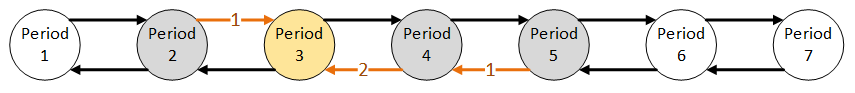
\includegraphics[width=\linewidth]{./flow_diagram}
	\caption{A flow diagram of a 7 period day for a particular teacher. The grey and yellow nodes represent periods in which the teacher is scheduled; the yellow node represents the sink. Black arrows are possible flow avenues between adjacent nodes; those that are experiencing flow are labelled with their flow value. For example, period five contributes a flow of 1 to period four, which therefore contributes a total of 2 (1 from period five, plus an additional 1), which drains into the sink located at period three.}
	\label{fig:flow-diagram}
\end{figure}

\subsection{PE Requirement}

The second iteration of our model increased the number of periods including lunch from 7 to 8 (or, excluding lunch, 6 to 7) and required that every student take one PE course a day. Moving from 6 class periods of 55 minutes each to 7 periods of 45 minutes each allows students to take the same courses while additionally adding PE into their schedule. This is of course a trade-off;  shorter periods means less instructional time per period, but more periods overall. The PE requirement is formulated as follows:

% PE every day
\begin{equation} \label{eq:one-sink}
	\displaystyle\sum_{c,p} X_{s,c,p} \cdot PE_{c} = 1 \quad \forall s
\end{equation}

A similar constraint ensured that students could only be enrolled in PE classes corresponding to their particular grade level (i.e. sixth graders can only take PE6, and so on).

Some space requirement also come into play when scheduling PE. In this particular school, there are two locations in which PE can be held. One of them is the cafeteria, and is therefore unavailable during lunch periods, the periods adjacent to lunch periods due to prep time and cleanup, and first period due to assemblies and breakfast cleanup. Therefore, we require that at maximum only one section of PE can be scheduling during these periods.

% restrict PE periods
\begin{equation} \label{eq:one-sink}
	\displaystyle\sum_{t} Y_{t,c,p} \leq 1 \quad \forall c \in PE, p \in U
\end{equation}

where $PE$ is the set of PE courses and U is the set of periods unavailable for multiple sections of PE (i.e. for an 8 period day, $U=\{1,3,4,5,6\}$ because lunch is scheduled during periods 4 and 5).


\section{Objectives}

\subsection{Electives}

This objective seeks to maximize the number of students assigned to the same electives they are currently taking. This is accomplished by counting the number of electives a student is assigned to in the solution that they are currently taking:

\begin{equation} \label{eq:link-num-electives}
	\text{objective:}\quad max \displaystyle\sum_{c,p} X_{s,c,p} \cdot (1-core_{c}) \cdot enrolled_{s,c} \quad \forall s
\end{equation}

We maximize the number of electives students are taking in the model solution that they are currently taking. Of course, this could be easily modified to maximize for elective preference as well (i.e. we are essentially using what students are currently taking as a proxy for how they might rank their desired electives; although this might be in reality a poor assumption, it is convenient from a data-gathering and modeling perspective).

\subsection{Additional PE teachers}

This objective seeks to minimize the additional amount of FTE (one full-time equivelent is equal to 40 hours per week) for PE teachers required when implementing the new PE mandate. In our data set, we created a number of ``mock'' PE teachers at varying levels of FTE; the solver could use these teachers in order to ensure every student was scheduled for PE. Additionally, the number of periods was increased rom 7 to 8. We minimized the additional FTE needed as follows:

\begin{equation} \label{eq:min-PE-FTE}
	\text{objective:}\quad min \displaystyle\sum_{t \in PE} Z_{t} \cdot FTE_{t}
\end{equation}

Objective expression \ref{eq:min-PE-FTE} is trivially weighted with objective expression \ref{eq:link-num-electives} in order to implement a multi-objective optimization problem. In general, we weighted objective expression~\ref{eq:min-PE-FTE} higher in order to ensure the least amount of additional FTE was needed.

\section{Results}

\subsection{Model Tractability}

The initial model (i.e. solving without the PE requirement) had a total of 108846 rows and 200519 columns, most of which were binary. With the PE requirement, the model had a total of 129235 rows and 229253 columns. When solving the initial model, Gurobi had difficulty finding initial feasible integer solutions without the use of heuristics. Ultimately, we virtually always used the ``feasibility pump'' \cite{Fischetti2005} heuristic in order to find an initial feasible integer solution.

The models were run on an Intel Xeon E3-1240 CPU using all 8 threads. The initial model reached 0.19\% of proven optimality within 47 minutes; an additional 70 minutes of runtime failed to improve the incumbent solution. With the PE requirement, the model reached proven optimality in 60 minutes.

\subsection{Model Results}

\begin{figure}
\centering
	% [width=8cm] 
	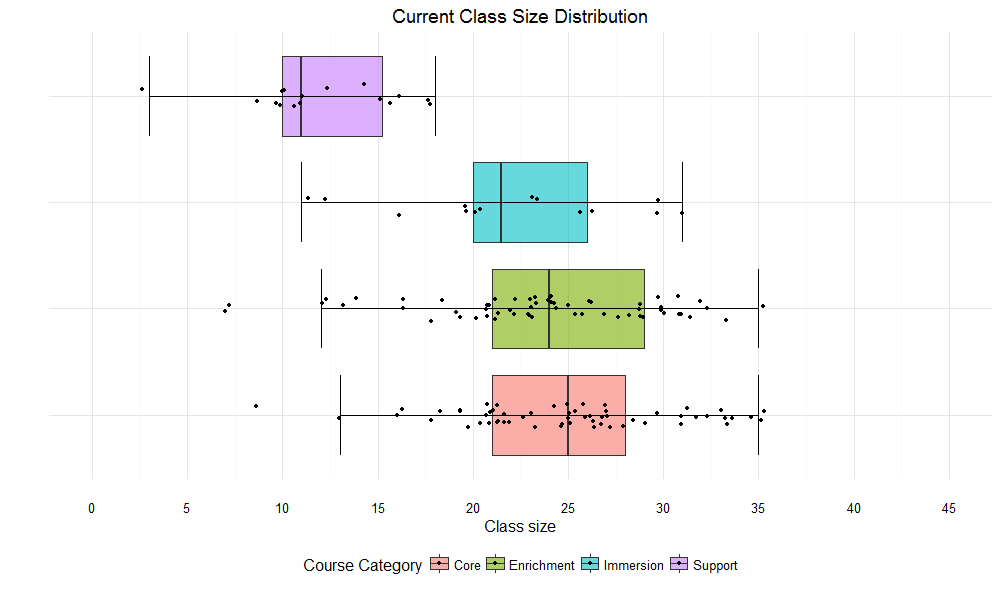
\includegraphics[width=\linewidth]{./current_class_size_distribution}
	\caption{The current class size distribution. There are some classes above 30 students, something parents expressed concern over in various community meetings.}
	\label{fig:current-class-size-distribution}
\end{figure}

\begin{figure}
\centering
	% [width=8cm] 
	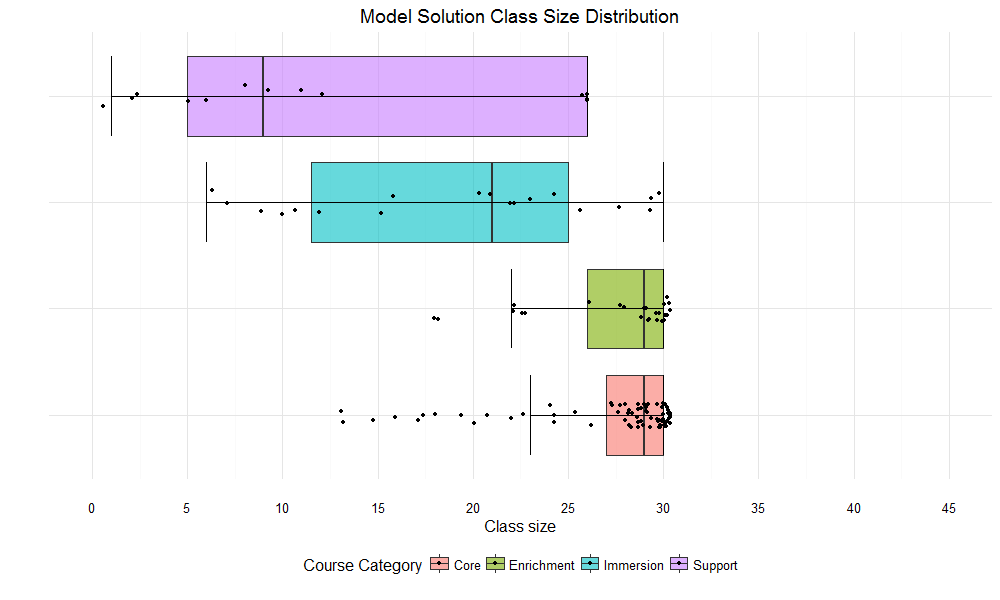
\includegraphics[width=\linewidth]{./model_solution_class_size_distribution}
	\caption{The class size distribution produced by the optimization model. There are no longer any classes above 30 students.}
	\label{fig:model-class-size-distribution}
\end{figure}

As can be seen by comparing figure~\ref{fig:current-class-size-distribution} and figure~\ref{fig:model-class-size-distribution}, the optimization model produces a solution in which no classes are enrolled with more than 30 students. However, this comes at a trade-off; table~\ref{tab:num-electives-lost} shows the number of students who are no longer able to take electives they are currently enrolled in. 372 students are taking all their current electives; 153 students are no longer taking one of their current electives; and 16 students are no longer taking two of their current electives.

\begin{table}[]
\centering
\caption{The number of students who are no longer taking electives they are currently enrolled in. 372 students are taking all their current electives; 153 students are no longer taking one of their current electives; and 16 students are no longer taking two of their current electives.}
\label{tab:num-electives-lost}
\begin{tabular}{ll}
\hline
Current Electives Lost & Number of Students \\ \hline
0                      & 372                \\
1                      & 153                \\
2                      & 16                 \\ \hline
\end{tabular}
\end{table}

This intuitively makes sense; as we decrease the maximum allowed class size, fewer students are able to take popular electives and must be displaced. One solution might be to hire more teachers for a desireable elective, or increase specific class sizes based on demand and expected educational impact.

\section{Discussion and Future Work}

Our two major objectives---minimizing class size and scheduling PE---are achieved. This helps demonstrate that using a Mixed Integer Programming model is a timely and effective method for scheduling a middle school. More generally, this model addresses a major need of school schedulers, namely the ability to quickly prototype different scheduling criteria. Hopefully it is clear how versitile a mathematical programming approach is---additional constraints and objectives could be easily implemented to model other outcomes administrators desire.

Future work lies in two major domains. Firstly, a number of modeling improvements could be made, such as explicitly scheduling courses into individual rooms. In addition to students ranking the courses they would like to take, teachers could analagously rank the courses they would like to teach. Objective functions could be designed to ensure teachers are, as much as is possible without limiting student preference, able to teach the courses they prefer. Additionally, an objective function could be implemented to get class sizes to specific targets, rather then simply limiting class sizes with an upper and lower bound. Lastly, lots of symmetry exists in the current model formulation. The model currently doesn't differentiate between students who have preference for the same elective. This symmetry could be broken by weighting students' preferences in some fashion, for example.

Secondly, a significant task lies in convincing school administrators and scheduling teams to adopt a mathematical programming approach to school scheduling rather then relying on heuristic measures. While certainly adequate, these methods fall short of delivering an optimal course schedule that maximizes student preference while ensuring appropriate class sizes.

\section*{Acknowledgement}

We'd like to thank Shawn Helm at Portland Public Schools for his general guidance and savvy model-building and Professor Tim Anderson, Ph.D. at Portland State University for his counsel, constructive criticism, and assistance in model formulation.

\bibliography{./education-scheduling-mip-model-paper}
\bibliographystyle{plain}

\end{document}






